
\documentclass[letterpaper,english,10pt]{article}

\usepackage{%
	amsfonts,%
	amsmath,%	
	amssymb,%
	amsthm,%
	babel,%
	bbm,%
	%biblatex,%
	caption,%
	centernot,%
	color,%
	enumerate,%
	%enumitem,%
	epsfig,%
	epstopdf,%
	etex,%
	fancybox,%
	framed,%
	fullpage,%
	%geometry,%
	graphicx,%
	hyperref,%
	latexsym,%
	mathptmx,%
	mathtools,%
	multicol,%
	pgf,%
	pgfplots,%
	pgfplotstable,%
	pgfpages,%
	proof,%
	psfrag,%
	%subfigure,%	
	tikz,%
	times,%
	ulem,%
	url,%
	xcolor,%
	mathpazo
}

\definecolor{shadecolor}{gray}{.95}%{rgb}{1,0,0}
\usepackage[margin=1in,top=0.75in]{geometry}
\usepackage[mathscr]{eucal}
\usepgflibrary{shapes}
\usepgfplotslibrary{fillbetween}
\usetikzlibrary{%
  arrows,%
  backgrounds,%
  chains,%
  decorations.pathmorphing,% /pgf/decoration/random steps | erste Graphik
  decorations.text,% 
  matrix,%
  positioning,% wg. " of "
  fit,%
  patterns,%
  petri,%
  plotmarks,%
  scopes,%
  shadows,%
  shapes.misc,% wg. rounded rectangle
  shapes.arrows,%
  shapes.callouts,%
  shapes%
}

%\pgfplotsset{compat=newest} %<------ Here
\pgfplotsset{compat=1.11} %<------ Or use this one

\theoremstyle{plain}
\newtheorem{thm}{Theorem}[section]
\newtheorem{lem}[thm]{Lemma}
\newtheorem{prop}[thm]{Proposition}
\newtheorem{cor}[thm]{Corollary}
\newtheorem{clm}[thm]{Claim}

\theoremstyle{definition}
\newtheorem{axiom}[thm]{Axiom}
\newtheorem{defn}[thm]{Definition}
\newtheorem{conj}[thm]{Conjecture}
\newtheorem{exmp}[thm]{Example}
\newtheorem{exerc}[thm]{Exercise}
\newtheorem{assum}[thm]{Assumptions}

\theoremstyle{remark}
\newtheorem{rem}[thm]{Remark}
\newtheorem{note}[thm]{Note}

\newcommand{\Cov}{\operatorname{Cov}}
%\newcommand{\det}{\operatorname{det}}
\newcommand{\Real}{\mathbb{R}}
\newcommand{\tr}{\operatorname{tr}}
%\newcommand{\Var}{\operatorname{Var}}

\DeclareMathOperator{\sign}{sign}
%\renewcommand{\proof}[1]{\begin{proof}#1\end{proof}}
\newcommand{\EQ}[1]{\begin{equation*}#1\end{equation*}}
\newcommand{\EQN}[1]{\begin{equation}#1\end{equation}}
\newcommand{\eq}[1]{\begin{align*}#1\end{align*}}
\newcommand{\meq}[2]{\begin{xalignat*}{#1}#2\end{xalignat*}}
\newcommand{\norm}[1]{\left\lVert#1\right\rVert}
\newcommand{\abs}[1]{\left\lvert#1\right\rvert}
\newcommand{\expect}[1]{\mathbb{E}\left[{#1}\right]}
\newcommand{\prob}[1]{\mathbb{P}\left[{#1}\right]}
\newcommand{\given}{\; \big\vert \;} 
\newcommand{\set}[1]{\left\{#1\right\}} 
\newcommand{\indicator}[1]{\mathbb{1}_{\set{#1}}} 
\newcommand{\inner}[1]{\left\langle#1\right\rangle}
\newcommand{\red}[1]{\textcolor{red}{#1}} 
\newcommand{\E}[1]{\mathbb{E}\left[#1\right]}
\newcommand{\Var}[1]{\operatorname{Var}\left[#1\right]}

\newcommand{\D}{\mathbb{D}}
%\newcommand{\E}{\mathbb{E}}
\newcommand{\N}{\mathbb{N}}
\renewcommand{\P}{\mathbb{P}}
\newcommand{\Q}{\mathbb{Q}}
\newcommand{\R}{\mathbb{R}}
\newcommand{\Z}{\mathbb{Z}}

\newcommand{\bU}{\mathbf{1}}
\newcommand{\bx}{\mathbf{x}}

\newcommand{\cB}{\mathcal{B}}
\newcommand{\cC}{\mathcal{C}}
\newcommand{\cD}{\mathcal{D}}
\newcommand{\cF}{\mathcal{F}}
\newcommand{\cG}{\mathcal{G}}
\newcommand{\cH}{\mathcal{H}}
\newcommand{\cO}{\mathcal{O}}
\newcommand{\cT}{\mathcal{T}}
\newcommand{\cX}{\mathcal{X}}
\newcommand{\cY}{\mathcal{Y}}

\newcommand{\sA}{\mathscr{A}}
\newcommand{\sB}{\mathscr{B}}
\newcommand{\sC}{\mathscr{C}}
\newcommand{\sD}{\mathscr{D}}
\newcommand{\sE}{\mathscr{E}}
\newcommand{\sF}{\mathscr{F}}
\newcommand{\sG}{\mathscr{G}}
\newcommand{\sH}{\mathscr{H}}
\newcommand{\sL}{\mathscr{L}}
\newcommand{\dO}{\mathscr{O}}
\newcommand{\sS}{\mathscr{S}}
\newcommand{\sT}{\mathscr{T}}
\newcommand{\sX}{\mathscr{X}}
\newcommand{\sY}{\mathscr{Y}}
\newcommand{\sZ}{\mathscr{Z}}

% Debug
\newcommand{\todo}[1]{\begin{color}{blue}{{\bf~[TODO:~#1]}}\end{color}}

% a few handy macros

\renewcommand{\le}{\leqslant}
\renewcommand{\ge}{\geqslant}
\newcommand\matlab{{\sc matlab}}
\newcommand{\goto}{\rightarrow}
\newcommand{\bigo}{{\mathcal O}}
%\newcommand{\half}{\frac{1}{2}}
%\newcommand\implies{\quad\Longrightarrow\quad}
\newcommand\reals{{{\rm l} \kern -.15em {\rm R} }}
\newcommand\complex{{\raisebox{.043ex}{\rule{0.07em}{1.56ex}} \hskip -.35em {\rm C}}}


% macros for matrices/vectors:

% matrix environment for vectors or matrices where elements are centered
\newenvironment{mat}{\left[\begin{array}{ccccccccccccccc}}{\end{array}\right]}
\newcommand\bcm{\begin{mat}}
\newcommand\ecm{\end{mat}}

% matrix environment for vectors or matrices where elements are right justifvied
\newenvironment{rmat}{\left[\begin{array}{rrrrrrrrrrrrr}}{\end{array}\right]}
\newcommand\brm{\begin{rmat}}
\newcommand\erm{\end{rmat}}

% for left brace and a set of choices
%\newenvironment{choices}{\left\{ \begin{array}{ll}}{\end{array}\right.}
\newcommand\when{&\text{if~}}
\newcommand\otherwise{&\text{otherwise}}
% sample usage:
%  \delta_{ij} = \begin{choices} 1 \when i=j, \\ 0 \otherwise \end{choices}


% for labeling and referencing equations:
\newcommand{\eql}{\begin{equation}\label}
\newcommand{\eqn}[1]{(\ref{#1})}
% can then do
%  \eql{eqnlabel}
%  ...
%  \end{equation}
% and refer to it as equation \eqn{eqnlabel}.  


% some useful macros for finite difference methods:
\newcommand\unp{U^{n+1}}
\newcommand\unm{U^{n-1}}

% for chemical reactions:
\newcommand{\react}[1]{\stackrel{K_{#1}}{\rightarrow}}
\newcommand{\reactb}[2]{\stackrel{K_{#1}}{~\stackrel{\rightleftharpoons}
   {\scriptstyle K_{#2}}}~}


\makeatletter
\def\th@plain{%
  \thm@notefont{}% same as heading font
  \itshape % body font
}
\def\th@definition{%
  \thm@notefont{}% same as heading font
  \normalfont % body font
}
\makeatother
\date{}

\graphicspath{{./Figures/}}
%\usepackage{witharrows}

%\usepackage{multirow}
%\usepackage{booktabs}
%\usepackage{amssymb}

%opening
\title{Lecture-26: Analysis of Medium Access Control algorithms over computer networks using mean field limits}
%\author{Ajay Kumar Badita, Ankit Dhiman}

\begin{document}
\maketitle
\section{Introduction}

Consider N users (or computers) communicating in a wired or wireless Local Area Network (LAN). To transmit data packets, users have to share a single resource (a cable in wired LANs or a radio channel in wireless LANs) using some Medium Access Control (MAC) protocols. \\

These protocols are distributed, meaning that each user runs its protocol independently of the other users sharing the same resource. This architecture has ensured the scalability of LANs (in the sense that new users can join and leave the network without the need of explicitly advertising it); it has played a crucial role in their development and hence contributed to the rapid growth of the Internet.\\

When two users cannot simultaneously successfully transmit data packets (because they share the same resource), we say that these users interfere. Two interfering users who simultaneously transmit experience a collision, and the packets have to be retransmitted. \\

Most current MAC protocols limit collisions using the following two main principles:

\begin{itemize}

\item First, before transmitting, users sense the resource and should it be busy they abstain from transmitting. This technique is referred to as CSMA (Carrier Sense Multiple Access) and ensures that packet transmissions cannot be interrupted. Even if the sensing mechanism is perfect, a collision may still occur if two interfering users start transmitting at the same time (or rather so close together in time that CSMA can’t prevent the collision). 

\item  The second main principle, termed random back-off, aims at reducing the possibilities that several users start transmitting simultaneously. To do so, a user only starts transmitting with a certain probability less than one. This probability is adapted to the number of successive collisions experienced by users, which allows users to infer the level of congestion of the resource.\\

\end{itemize}

Typically, in LANs today, users implement the exponential back-off algorithm (also referred to as the Decentralized Coordination Function (DCF) in the standards): the transmission probability is divided by a factor two after each collision, and it is reinitialized after the successful transmission of a packet.\\

The performance of MAC protocols is measured in terms of the throughput realized by the various users, i.e., of the number of packets successfully transmitted by users per second. \\

The performance analysis requires that we can characterize the joint evolution of the transmission probabilities of the N users.\\

These probabilities evolve according to a N-dimensional Markov chain that is usually intractable because of the correlations introduced by collisions. Mean field asymptotics are useful to approximate this evolution.\\

We consider networks with full interference where all pairs of users interfere, and networks with partial interference where users do not interfere with all other users. In the latter scenario, users are classified according to the set of users they interfere with. Partial interference typically arises in wireless networks as illustrated in Figure 1:
 
\begin{figure}[h!] 
	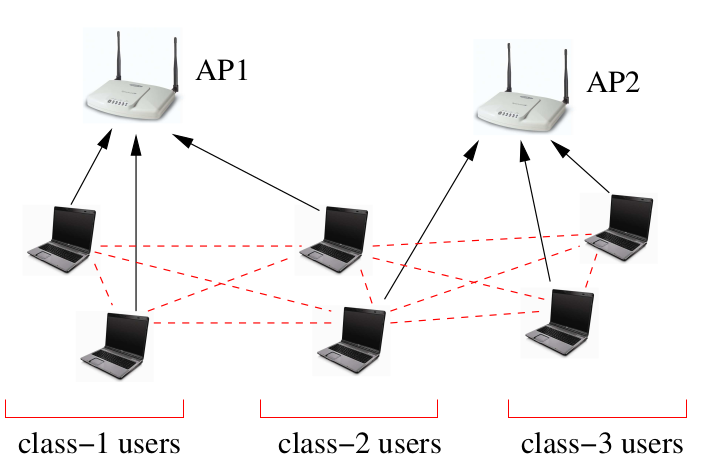
\includegraphics[width=\linewidth]{L26_Fig_1.png}
	\caption{A network with partial interference - A dashed line between two
users means that they sense each other.}
	\label{fig:1}
\end{figure} 

All 6 users are willing to transmit data packets to the access points 1 or 2; class-1 (resp. class-3) users interfere with users of classes 1 and 2 (resp. 2 and 3), whereas class-2 users interfere with all users. Two users of class 1 and 3 respectively can not sense each
other.

\section{System model}

We consider for example Local Area Networks (LANs) which are computer networks with relatively small geographic coverage (an office, a house, a part of a campus), and which constitutes the first crucial component of the Internet. \\

Transmissions in LANs are handled either on a cable (wired LANs) or on a radio channel (wireless LANs, also commonly called WiFi). Here we will focus on wireless LANs (analysis can be carried out similarly in the case of wired LANs). \\

In wireless LANs, users that are close to each other or that wish to transmit to the same receivers interfere in the sense that they cannot simultaneously transmit packets successfully. Two interfering users transmitting simultaneously are said to experience a collision. A collision is detected by a user at the end of the packet transmission when the corresponding receiver does not acknowledge a successful reception. \\

One of the most challenging problem in computer networking has been to design mechanisms so that interfering users could efficiently and fairly share the resource in a distributed manner.\\

\subsection{Random back-off algorithms} Currently the DCF is a version of the classical binary exponential back-off algorithm: after each successful transmission, a user picks a back-off counter uniformly in $\{0, . . . , t_{min}\}$, and after $m$ successive collisions uniformly in $\{0, . . . , 2^mt_{min}\}$.\\

In the following, we assume that the back-off distribution is always geometric (so as to keep a simple Markovian setting), although we could easily generalize the analysis to uniform distributions. With this assumption, each user transmits with a given probability $p$ at the beginning of each idle slot.
We consider the following generic way of adapting this probability: first the probability belongs to a countable set $\mathbb{B}$, after a successful transmission $p$ is updated to $S(p)$, and after a collision $p$ is updated to $C(p)$, where $S(·)$ (resp. $C(·)$) is a decreasing (resp. increasing) mapping from $\mathbb{B} \to \mathbb{B}$. Let $p_0 = \max\{p \in \mathbb{B}\}$.

\subsection{Interference model and user class} We consider a simple model for interference as follows: first, the N users
are classified according to their interference properties, i.e., two users belong to the same class if they interfere with (resp. are interfered with and by) the same set of users. Two users are of the same class if the corresponding links are located in the same geographic region (see for example the network of Figure 1). \\

Denote by $\mathbb{C}$ the set of user classes, and by $\mu_c$ the proportion of users of class $c$. $i \in c$ denotes the fact that user $i$ is of class $c$. Then interference between users of different classes is characterized by the inci-
dence matrix $A$ such that $A_{cd} = 1$ if class-c users interfere class-d users, and $A_{cd} = 0$ otherwise. 
Denote by $V_c = \{d \in C : A_{cd} = 1\}$ the set of classes of links interfering with class-$c$ links.
We say that the network has full interference if $A_{cd} = 1$ for all $c, d \in \mathbb{C}$ and has partial interference otherwise.

\subsection{Performance metrics}The performance metrics we aim at analyzing is the long-term throughput (the number of packets successfully transmitted per time unit) achieved by the users of various classes. We denote by $\gamma_c$ the throughput of class-$c$ users.\\

Deriving expressions for this performance metrics is notoriously difficult. This is due to the inherent interactions between users through interference.\\

In case of full interference, the network can be modeled as a simple system of particles with no randomly varying environment. However, to analyze a network with partial interference, the introduction of this varying environment is necessary.\\

\subsection{Model analysis}We consider a network of $N$ users and analyze the system at the beginning of each slot. Denote by $p_N
^i (k)/N$ the probability user $i$ becomes active at the end of the $k$-th slot, if idle (note the normalization of this probability by $1/N$ to be able to conduct the asymptotic analysis when $N$ grows large). For all $i, k, N , p_N^i (k) \in \mathbb{B}$.\\

To capture the network dynamics, we define a process $Z_N = \{Z_N (k), k \geq 0\}$ representing the state of classes during slot $k$. $Z_c^N (k) \in \{0, 1, 2\}$, where $Z_ c(k) = 0$ if and only if there is no transmitting user of class $c$, $Z_c^N (k) = 1$ if
and only if there is one successfully transmitting user of class c and $Z_c^N (k) = 2$ if and only if there is at least one user of class c currently in collision with another user in $V_c$ . Let $Z = \{0, 1, 2\}^{|C|}$ denote the state space of $Z$. We introduce the clear-to-send functions $C_c$ as follows : If $Z^N (k) = z$, a class-$c$ link is clear to send at the end of slot $k$ and $C_c (z) = 1$ if $z_d = 0$ for $d \in V_c$, otherwise $C_c (z) = 0$.\\

Modelling the network as $N$-particles system, the $i$-th user corresponds to the $i$-th particle with state describing the class of the user and the transmission probability at the end of the next idle slot $X_i^N (k) = (c_i , p^N_i (k)) \in \mathbb{X} = \mathbb{C} \times \mathbb{B}$.\\

The environment process: the evolution of the environment is determined by the states of all the particules through $v^N$ . The evolution of the $i$-th particle depends on whether or not the corresponding user senses the channel idle or not, i.e., $Z_i^N (k) = Z_c^N (k)$ for $i \in c$.

\subsection{Particle transitions} We first compute the transition probabilities for the various particles. The set $S$ of possible transitions is composed by two functions, the first one representing a successful transmission $p \to S(p)$ and the other one collisions $p \to C(p)$. Note that the class of a particle/user does not change.\\

Let $v_c^N (k) = \frac{1}{N}\sum_{i =1}^{N} \delta_{p_i^N(k)} \mathbb{1}_{c(i)=c}$ and $v^N (k) = (v_c^N (k))_{c\in\mathbb{C}}$.\\

Assume that at some slot $k$, the system is in state: \EQ{((c^N_i (k), p_i^N (k))_{i=1,...N}, v^N(k), Z^N(k))) = ((c_i, p_i )_{i=1,...,N} , \alpha, z)}

A class-$c$ user $i$ may have a transition at the end of slot $k$ only if $C_c (z) = 1$. In this case it can either initiate a successful transmission or experience a collision. If $C_c (z) = 1$, the event that none of the users in $c$ transmits at the end of slot $k$ is given by $D_c^N = \prod_{i \in c}{\mathbb{1}_{(NU_i > p_i)}} $, where the $U_i$ ’s are i.i.d. r.v. uniformly distributed on $[0, 1]$.\\

The event that user $i \in c$ accesses the channel with success at the end of slot $k$ is given by the indicator:
\EQ{\mathbb{1}_{\{NU_i \leq p_i\}}C_c(z)\prod_{j \in c,j \neq i}{\mathbb{1}_{\{NU_j > p_j\}}}\prod_{d \in V_c ,d \neq c}{(C_d(z)D_d^N + (1 - C_d (z)))}}

Averaging the above quantity gives the transition probability $F_S^N((c, p_i ), \alpha, z)/N$ corresponding to a successful transmission. For all $\alpha \in P(\mathbb{B})$ and all $f$ $B$-valued functions, define $\langle f, \alpha \rangle =  \sum_{p}f(p)\alpha(p)$. Moreover let $\alpha_c$ denote the restriction of $\alpha$ to users of class $c$. Let $I$ denote the identity function. Then:

\EQ{F_S^N ((c, p_i ), \alpha, z) =\frac{p_i}{1-\frac{p_i}{N}}C_c(z)\prod_{d in V_c}{(C_d(z)(e^{\langle Nlog(1− \frac{1}{N}),\alpha_d\rangle}- 1) + 1)}} 

Similarly, the event that user $i \in c$ experiences a collision at the end of slot $k$ is given by the indicator:
\EQ{\mathbb{1}_{\{NU_i \leq p_i\}}C_c(z)(1-\prod_{j \in c,j \neq i}{\mathbb{1}_{\{NU_j > p_j\}}\prod_{d \in V_c,d \neq c}{(C_d(z)D_d^N + (1-C_d(z)))}}}
and the transition probability $F_C^N((c, p_i ), \alpha, z)/N$ corresponding to a collision reads:
\EQ{F^N_C((c, p_i), \alpha, z) = p_iC_c(z)(1 -\frac{1}{1 - \frac{p_i}{N}}\prod_{d \in V_c, d \neq c}{(C_d(z)(e^{\langle Nlog(1-\frac{1}{N},\alpha_d\rangle} - 1) + 1)})}
We also need to introduce a virtual transition from $(c, p)$ to $(c, p)$ with transition rate $F^N_{\phi}((c, p_i), \alpha, z) = 1 - p_iC_c(z)$. 
With this virtual transition the sum of the transition rates sums to 1.\\

Since $Nlog(1-x/N)$ converges to $-x$, we obtain the following expressions for the asymptotic transition rates, $F_\phi((c, p_i), \alpha, z) = 1 - p_iC_c(z)$,
\EQ{F_S((c, p_i), \alpha, z) = p_iC_c(z)\prod_{d \in V_c}{(C_d(z)(e^{-\langle I,\alpha_d \rangle} - 1) + 1)}}
\EQ{F_C((c, p_i), \alpha, z) = p_iC_c(z)(1 -\prod_{d \in V_c}{(C_d(z)(e^{-\langle I,\alpha_d \rangle} - 1) + 1)}}

\subsection{Stationary throughputs}We are interested in deriving the stationary throughputs achieved by users of various classes. 
To do so, we derive the stationary distribution $Q_{st}$ and $\pi_{Q_{st}}$ of the particles and the background process.\\

To simplify the notation we write $Q_{st} = Q$ and $\pi_Q = \pi$. Also denote $Q^p_c = Q({c, p})$ the stationary proportion of users of class $c$ transmitting with probability $p$.\\

Consider the point process of returns to the set $A = \{z : C_c(z) = 1\}$. Let $T_1$ denote the first return time after time zero. 
%By the cycle formula (see
%(1.3.2) in [5]) we may express the steady state probability of a user in c successfully
%transmitting a packet by the mean time spent in the transmission
%state per cycle divided by the mean cycle length. The expectation is calculated
%with respect to the Palm measure of the point process of returns to A
%but in this Markovian case this just means starting on A with probability
%πA which is π renormalized to be a probability on A.
A user in $c$ can only go into a successful transmission state once per cycle;i.e. no other user in $c$ transmits and other users in $V_c$ are either blocked or remain silent. Hence the mean time per cycle spent in a transmission state is \EQ{\sum_{z \in A}{\pi^A(z)Lg(z)}} where \EQ{g(z) = p_c\prod_{d \in V_c,d \neq c}{(C_d(z)(e^{-p_d} - 1) + 1)}}
Moreover,\EQ{\sum_{z \in A}{\pi^A(z)E_z[T_1]} = \frac{1}{\pi(A)}} i.e. the intensity of the point process of visits to $A$. Finally the total throughput of the users of class $c$ is \EQ{\gamma_c =\sum_{z:C_c(z)=1}\pi(z)Lp_c\prod_{d \in V_c}{C_d(z)(e^{-p_d} - 1) + 1}} where
\EQ{p_c =\sum_{p \in \mathbb{B}}pQ^p_c}
which can be interpreted as the probability that a user of class c attempts
to use the channel at the end of an empty slot.
%\section{Income inequality in pay distribution}
%Let us now focus on  the inequality in pay scale of employees in an organization. As of 2009 top 1\% of income earners received 17.2\% if income. Fundamental to solving this problem is understanding why this occurs. Clearly different employees make different contributions and this implies a certain amount of  inequality in income and wealth has to be expected. So we can ask the question what is a fair inequality? What kind of pay distribution will arise, under ideal conditions in a free market where employers are seeking profit maximization and employees are seeking utility maximization?
%
%\section{Connection between statistical physics and income inequality problem}
%There has been a lot of effort to model income and wealth distributions by applying statistical physics method. But appreciating those efforts there is still a conceptual gap between them. How will a theory of random particles with no intelligence be able to model a environment that consists of rational profit seeking agents? 
%
%\section{Game Theory}
%We will use theory of potential games as a tool for getting the equilibrium of income inequality problem. So lets take a brief introduction to game theory. \\
%Game theory is the study of mathematical models for strategic interaction between rational and intelligent agents. There are different types of games. Let us look at the one relevant to us which is strategic form games. Let us discuss a bit on what terms rational and intelligent means:
%
%\begin{defn}
%Strategic Form Game: A strategic form game $\Gamma$ is a tuple $\langle N, (S_i)_{i\in N}, (u_i)_{i \in N} \rangle$ , where 
%\begin{itemize}
%\item $N = \lbrace 1,2,\dots ,n\rbrace$ is set of players;
%\item $S_1,S_2,\dots S_n$ are sets called the strategy sets of the players $1,\dots , n$ respectively; and
%\item Set of strategy profiles $S$ is the cartesian product of individual strategy sets $S=\lbrace s_1 \times s_2 \times s_N : s_1\in S_1, s_2 \in S_2 \dots s_N \in S_N  \rbrace $
%\item $u_i  : S \rightarrow \R$ for $i=1,2,\dots n$ are mappings called the utility functions or payoff functions.
%
%\end{itemize}
% \end{defn}
%\begin{exmp}
%$ N=\lbrace 1,2 \rbrace ;S_1= S_2 = \lbrace A,B \rbrace ;$ \\ \\
%$u_1(A,A) = 10; u_1(A,B)=0; u_1(B,A) = 0 ; u_1(B.B) = 1;$ \\ \\
%$u_2(A,A) = 10; u_2(A,B)=0; u_2(B,A) = 0 ; u_2(B.B) = 1;$ \\ \\
%\end{exmp}
%Payoff functions of a player is not just dependent on his strategy but also on what strategies others are playing.
%Above example can be put in a tabular form
%
%\begin{table}[ht]
%\begin{center}
%\begin{tabular}{|c|c|c|}
%\hline
%\multirow{2}{*}{1} & \multicolumn{2}{c|}{2} \\ \cline{2-3} 
%                   & A           & B        \\ \hline
%A                  & 10,10       & 0,0      \\ \hline
%B                  & 0,0         & 1,1      \\ \hline
%\end{tabular}
%\end{center}
%\end{table}
%
%
%
%
%
%
%
%Here first value in payoff cell stands for first player and second value stands for second player.
%\begin{defn}
%Potential Game: A strategic form game is a potential game if there exists a function $\phi:S \to R $ such that 
%\begin{equation} \label{pgt}
%\phi(S')-\phi(S'') = u_i(S') - u_i(S'')~~
%\forall~i , \forall S', S'' \in 
%\end{equation}
%\end{defn}
%
%This means if we know $\phi$ we know the payoff matrix upto a offset. 
%\begin{thm}\label{pgtne}
%	In a potenital game strategy profile maximizing $\phi$ is a Nash equilbria.
%\end{thm}
%\begin{proof}
%	Now consider two strategy $s'$ and $s''$ profiles which differs only in strategy for player $i$.Also assume $s'$ maximizes $\phi$. So $\phi(s')-\phi(s'')>0$ . But from $\ref{pgt}$ we have $u_i(s')-u_i(s'')>0 \forall i$ Hence $s'$ is a Nash equilbria.
%\end{proof}
%So in potential game theory all we need to find a Nash equilbria is to maximize $\phi$ 
%\begin{exmp}
%	Consider a game and its potential $\phi$, assuming $\phi(A,A)=0$
%		\begin{table}[ht]
%	\begin{minipage}{0.5\textwidth}
%	\begin{center}
%		\begin{tabular}{|c|c|c|}
%			\hline
%			\multirow{2}{*}{1} & \multicolumn{2}{c|}{2} \\ \cline{2-3} 
%			& A           & B        \\ \hline
%			A                  & 1,2       & 2,3     \\ \hline
%			B                  & 4,5        & 6,7     \\ \hline
%		\end{tabular}
%	\label{game2}
%	\caption{Game}
%		\end{center}
%	\end{minipage}
%\begin{minipage}{0.5\textwidth}
%	\begin{center}
%		\begin{tabular}{|c|c|c|}
%			\hline
%			\multirow{2}{*}{1} & \multicolumn{2}{c|}{2} \\ \cline{2-3} 
%			& A           & B        \\ \hline
%			A                  & 0     & 1      \\ \hline
%			B                  & 3        & 5    \\ \hline
%		\end{tabular}
%	\label{potential2}
%	\caption{potential}
%	\end{center}
%\end{minipage}
%\end{table}
%
%\end{exmp}
%
%
%\section{Dynamics} \cite{fairentrop}
%
% Consider a company $A$ with:
%\begin{enumerate}
%	 \item Total salary budget $M$ 
%	 \item Total number of employees $N$
%	 \item $k$ levels of employment with value $v_i$ for $i^{th}$ level.Assume $v_i < v_j$ for $i<j$
%	 For example level $1$ could be a clerk and level $k$ be CEO.
%\end{enumerate}
%
%For our market we assume a simplified model of all companies have same  slary budget and total number of employees and number of levels of employment. Also assume market is a \textbf{free market}.
%If we give equal salary to all employees we will get a distribution as in Figure 1(a). Now employees who contribute a value above average will try to leave company since they are underpaid. This fill shift the curve towards right as in Figure 1(b).But now below average employees are overpaid. They will be more competition for this level and this shifts distribution towards left.
%Let us look at an example.
%\begin{figure}[h!]
%	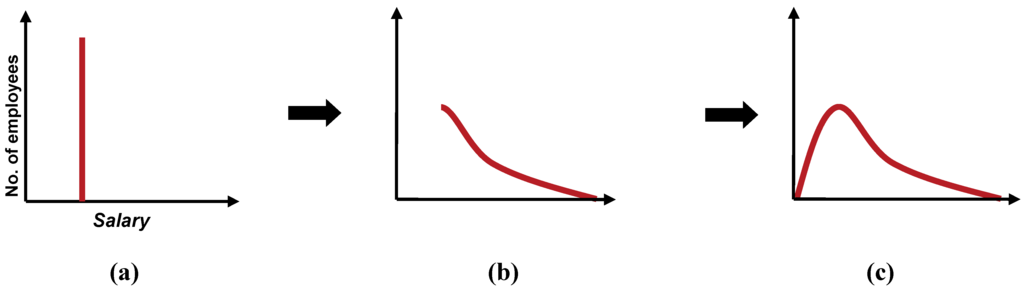
\includegraphics[width=\linewidth]{dbnR.png}
%	\caption{Evolving distribution}
%	\label{fig:1}
%\end{figure}
%
%Let us look at an example.
%\begin{exmp}
%	
%
%\begin{figure}[h!]
%	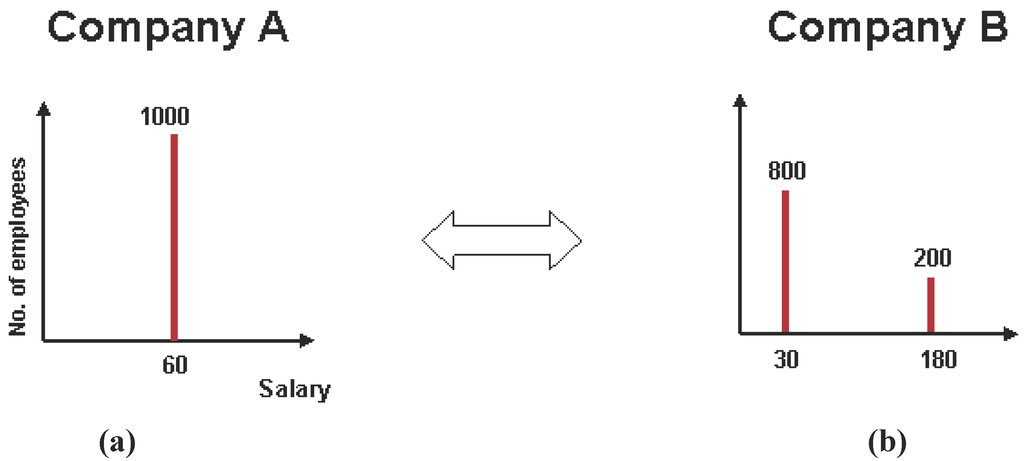
\includegraphics[width=\linewidth]{dynamics1.png}
%	\caption{Initial distribution}
%	\label{fig:2}
%\end{figure}
%
%Consider two companies A and B with 3 different levels of employment with $v1<v2<v3$; call it low skill, medium skill, high skill.
%Both A and B have $\text{total number of employees} ~ N =1000$ and $\text{total salary budget}~ M=\$60~ \text{million dollar}$ with initial distribution as shown in Figure 2 \ref{fig:2}.
%
%\begin{figure}[h!] 
%	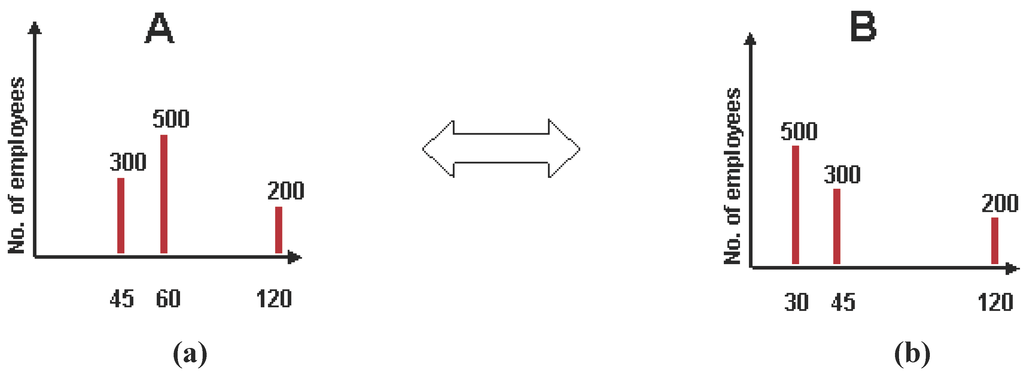
\includegraphics[width=\linewidth]{dynamics2.png}
%	\caption{Evolving}
%	\label{fig:3}
%\end{figure}
%
% Now highly skilled employees in company A are not satisfied; so they try to jump to $B$. Now $B$ is also trying to make profit out of this situation. So $B$ doesn't want to give the same salary of $180$  to highly skilled employees from $A$. But highly skilled employees from $A$ and $B$ will have a negotiation and say they settle for $120$. Now highly skilled employees of $A$ will be ready to work for $120$. Hence a new level will be formed both in $A$ and $B$ of $120$. Now distribtuion will look as given in Figure 3 \ref{fig:3}.
% 
% Now there could be a similar adjustment for mid level and low level employees. And final distribution will look like as Figure 4 \ref{fig:4}
%
%
%
%
%
%\begin{figure}[h!] 
%	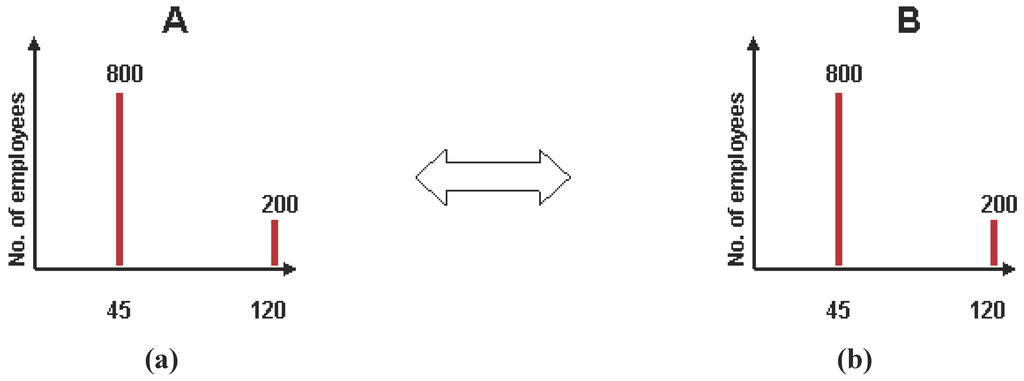
\includegraphics[width=\linewidth]{dynamics3.png}
%	\caption{After evolution}
%	\label{fig:4}
%\end{figure}
%
%So this is the dynamics we are talking about.
%\end{exmp}
%
%\section{Setting the payoff or utility}
%In general an employee feels they could be doing better given their talent and experience. Utility maximizing, fairness-seeking, teleological agents are always restless. Even though utility obtained by an employee is a complex aggregate, we formulate it as obtained from 3 major factors. 
%\begin{itemize}
%    \item Utility derived from salary.
%    \item Disutility from effort
%    \item Utility from fairness.
%    
%\end{itemize}
%\subsection{A note on fairness}
%Employees are looking for fair compensation for their abilities and contribution to the organization. This will depend on the education and other qualifications the possess. But an employee is looking for appreciation with respect to peers at his level. This means a clerk is not eyeing for the post of a CEO. Similarly a a vice president is not happy if he gets more salary than a clerk. But he expects to get utility on par with other vice presidents. So that means utility from fairness is a function only of number of employees at his level ($N_i$) . 
%\subsection{Functional form for utility terms}
%So we can write \\
%$h_i(S_i,E_i,N_i) = u(S_i) - v(E_i) + f(N_i)$
%$h_i$ : is the total utility of an employee earning a salary $S_i$ by expending an effort $E_i$ while competing with $(N_i -1) $ other agents. \\
%
%Now we need to come up with functional form for each of the three terms $u,v,f$ \\
%Let us consider the following empirical and theoretical considerations from literature regarding effort $E$ and salary $S$.
%\begin{itemize}
%\item Salary
% \begin{itemize}
%    \item Logarithmic function is commonly used in literature for utility from salary. 
%       
%    \item This gives $u(S_i) = \alpha ln S_i$
%       
%   \end{itemize}
%\item Effort 
%   \begin{itemize}
%    \item  Work by Katz \cite{katz} and Akerlof \cite{akerlof} gives following conditions to be satisfied by effort $E$ as a function of salary $S$
%    \begin{itemize}
%        \item $dE/dS >0$
%        \item $E(0) \leq 0 $
%        \item the elasticity $S/E \times (dE/dS)$ should be decreasing.
%    \end{itemize}
%    \item Empirical evidence that supports effort $E$ correlates with $lnS$ ; $E= lnS$; given in Stratton \cite{stratton} and Ahituv and Lerman \cite{ahituv}. This goes well with previous point because: \\
%     \begin{itemize}
%     \item $\frac{dE}{dS} = \frac{1}{S} >0$
%     \item $E(0) = -\inf < 0$
%     \item $S/E \times (\frac{dE}{dS}) = (\frac{S}{ln S}) \times \frac{1}{S} = \frac{1}{ln S} $ is decreasing.
%     \end{itemize}
%     \item Hence $v(E_i) = \beta (ln S_i)^2$
%   \end{itemize}
%   \item Fairness 
%        \begin{itemize}
%        \item We propose $f(N_i) = -\gamma~ ln N_i$
%        \item We note following observations are captured in this form
%           \begin{itemize}
%               \item As $N_i \to \inf $, $f_i \to -inf$; this captures the idea that when there are too many employees working with a person his appreciation is minimized.
%               \item When $N_i = 0, f_i \to \inf. $ This explains why employees are in constant search of their dream jobs. When $N_i=0$ , this is when utility from fairness is maximized mathematically; but this cannot be attained in reality because minimum value of $N_i$ is 1 in reality (at least  oneself should be there).
%           \end{itemize}
%        \end{itemize}
%   
%\end{itemize}
%Thus we have :
%\begin{equation}
%    u(S_i) = \alpha ln S_i
%\end{equation}
%\begin{equation}
%    v(E_i) = \beta (ln S_i)^2
%\end{equation}
%\begin{equation}
%f(N_i) = - \gamma ln N_i
%\end{equation}
%\begin{equation}\label{utility}
% h_i(S_i,E_i,N_i) = u(S_i) - v(E_i) + f(N_i)= \alpha ln S_i - \beta (ln S_i)^2 - \gamma ln N_i
% \end{equation}
%\section{Applying potential game theory to income inequality problem}
%\begin{defn}
%	We apply the definition of payoff in continuous potential game theory; this is different from discrete case but idea remains same that a single function to deal with the payoff function of all players. By definition of payoff
%	\begin{equation}
%	h_i(x) \equiv  \frac{\partial\phi(x)}{\partial x_i} 
%	\end{equation}
%	where $x_i$ is the fraction of people at $i^{th}$ level; giving
%\end{defn}
%
%\begin{equation} \label{potential}
%    \phi(x) = \sum_{i=1}^{k}\int{}{}h_i(x)dx_i
%\end{equation}
%\begin{equation}
%    \phi(x) = \phi_u + \phi_v + \phi_f + constant ; where
%\end{equation}
%From \ref{utility} and \ref{potential} we need to find potential corresponding to each term. For salary($u_i$) and effort($v_i$) integration is straight forward.
%\begin{equation}
%    \phi_u = \alpha \sum_{i=1}^{k}x_i lnS_i ;and
%\end{equation}
%
%\begin{equation}
%    \phi_v = -\beta \sum_{i=1}^{k} x_i(ln S_i)^2 ; and
%\end{equation}
%
%\begin{align}
%  \phi_f &= \sum_{i=1}^{k}\int{}{}h_i(x)dx_i \\
%         &= - \gamma \sum_{i=1}^{k}\int{}{}ln N_i dx_i \\
%         &= -\gamma \sum_{i=1}^{k}\int{}{} ln (Nx_i) dx_i \\
%         &=-\frac{\gamma}{N} \sum_{i=1}^{k}\int{}{} ln (Nx_i) d(Nx_i); but \int{}{} lnxdx = xlnx -x ~ and ~ln(x!) = xlogx -x ~ \text{which gives}\\
%         &=\frac{\gamma}{N} ln\frac{N!}{\prod_{j=1}^{k}(Nx_i)!}   
%\end{align}
%
%We can show that $\phi(x)$ is strictly concave: 
%\begin{equation}
%    \dfrac{\partial^2 \phi(x)}{\partial x_i^2}= \dfrac{-\gamma}{x_i}<0
%\end{equation}
%Therefore, a unique Nash equilbrium exists for this game; which is a maximizer for $\phi$ . \\
%To find maximizer $x_i$
%we use langrangian multiplier method with $L$ as langrangian and $\lambda$ as Langrange multiplier. Thus 
%\begin{equation}
%     L=\phi + \lambda(1-\sum_{i=1}{n}x_i)
%\end{equation}
%We solve system of equations given by
%\begin{equation}
%     \frac{\partial L}{\partial x_i} =0 ~ \forall i
% \end{equation}
% 
% We get 
% \begin{equation}
%    \alpha ln S_i-\beta (ln S_i)^2 - \gamma ln Nx_i - \lambda = 0
% \end{equation}
% giving
% \begin{equation}
%     x_i = e ^ {\alpha ln S_i - \beta (ln S_i)^2 - \gamma ln N -\lambda}
% \end{equation}
% which can be rearranged to get
% 
% \begin{equation}\label{fairpotential}
%     x_i = \dfrac{1}{S_i Z}exp(-\dfrac{(lnS_i - \dfrac{\alpha+\gamma}{2\beta})^2 }{\dfrac{\gamma}{\beta}})
% \end{equation}
% where 
% \begin{equation}
%     Z = N exp[\lambda/\gamma - \dfrac{(\alpha + \gamma)^2}{4\beta \gamma}]
% \end{equation}
% which is a \textbf{log-normal distribution}
% 
%
%\section{Deriving Boltzmann distribution using potential game theory}
%Let us define the payoff of particles in the thermodynamic game:
%
%\begin{equation}\label{thermogame}
%    h_i(E_i,N_i) = -\beta E_i - ln N_i
%\end{equation}
%where $E_i$ is the energy of a molecule in state $i$, $\beta=\frac{1}{kT}$, $k=1.3806488 \times 10^{-23} JK^{-1}$ is Boltzmann constant; and $T$ is temperature.
% Now from \ref{potential} we have 
% \begin{equation}
% \phi(x) = \frac{-\beta}{N}+ \frac{1}{N}ln\frac{N!}{\prod_{i=1}^{n}(Nx_i)!}
% \end{equation}
% We need to maximize $\phi(x)$ under constraint $\sum_{j=1}{k}x_j = 1$.
% Using Langrange multiplier method with L as Langrangian we have
% \begin{equation}
%     L=\phi + \lambda(1-\sum_{i=1}{n}x_i)
% \end{equation}
% For maximizing; we solve set of equations given by
% \begin{equation}
%     \frac{\partial L}{\partial x_i} =0 ~ \forall i
% \end{equation}
% We get 
% \begin{equation}
%     \beta E_i  - ln N - ln x_i -\lambda = 0 
% \end{equation}
% giving
% \begin{equation}
%     x_i = e ^ {\beta E_i  - ln N  -\lambda}
% \end{equation}
% Also $\sum_{j=1}^{k}x_j=1$; which gives
% \begin{equation}
%     x_i = \frac{x_i}{1} = \frac{x_i}{\sum_{j=1}^{k}x_j} = \frac{e ^ {\beta E_i  - ln N  -\lambda}}{\sum_{j=1}^{k}e ^ {\beta E_j  - ln N  -\lambda}}
% \end{equation}
% giving
% \begin{equation}
%     x_i = \frac{e^{-\beta E_i}}{\sum_{j=1}^{k}e^{-\beta E_i}}
% \end{equation}
% which is nothing but \textbf{Boltzmann Distribution}
% 
%\section{Replicator Dynamics}
%Consider the situation of people buying cars. We compare people buying an SUV and compact cars. Let us define the following payoff table constructed by considering the fact that when one SUV meets another SUV there is less space on road and less fuel efficiency. We consider  similar situation for an SUV and compact and compact and compact.
%
%\begin{table}[ht]
%\begin{center}
%\begin{tabular}{|c|c|c|}
%\hline
%%\multirow{2}{*}{1} & \multicolumn{2}{c|}{2} \\ \cline{2-3} 
%                   & SUV           & Compact        \\ \hline
%SUV                 & 2,2       & 2,0      \\ \hline
%Compact                  & 0,2         & 3,3      \\ \hline
%\end{tabular}
%\end{center}
%\end{table}
%As from the table it is observed that purchasing compact cars is better for users.But in reality number of SUVs are on rise. How do we explain this situation. But people are not purely rational. They have emotions and feelings as well.One thing they do out of emotions is to copy others. Also they are not completely out of rationality. So in  order to model this situation we use replicator dynamics.
%This is a simple model of evolution and prestige based learning in games. We explain this model through an example\\ 
%\subsection{Model Description through example}
%Consider a population of $N$ people divided into $k$ classes . Let $x_i(t)$ be the fraction of people belonging to class $i$ at time epoch $t$.  Tuple $(x_1(t),\dots x_k(t))$ define the state of the population at time epoch $t$. $\pi_i(t)$ is the expected payoff for a player when randomly matched with another player. This is clearly a function of payoff matrix and state of population. \\
%In the SUV and compact cars game if we have a population of $50\%$ SUVs and $50\%$ comapct cars, expected payoff for an compact car owner is \\
%\begin{equation}
%E=0.5\times U_c(C,C) + 0.5 \times U_s(C,S)
%\end{equation}
%$E=0.5\times U_c(C,C) + 0.5 \times U_s(C,S)$(C stands for compact and S stands for SUV) where $U_c$ is the utility function for compact.First term corresponds to $50\%$ chance of meeting an compact and similarly second term corresponds to $50\%$ chance of meeting an SUV. In the
%Also we have $\sum_{i=0}^{k}x_i(t) = 1 ~~ \forall t$
%Now we see the equation for evolution of population in replicator dynamics.
%\begin{equation}
%    x_i(t+1) = \frac{x_i(t)\pi_i(t)}{\sum_{j=i}^{k}x_j(t)\pi_j(t)}
%\end{equation}
%We calculate rate of change of $x_i$ i.e $x_i(t+1)-x_i(t)$  
%\begin{equation}
%    x_i(t+1) - x_i(t) =  \frac{x_i(t)\pi_i(t)}{\sum_{j=i}^{k}x_j(t)\pi_i(t)} -x_i(t)
%    = \frac{x_i(t)(\pi_i(t)-\sum_{j=i}^{k}x_j(t)\pi_i(t)}{\sum_{j=i}^{k}x_j(t)\pi_i(t)}
%\end{equation}
%Denote by $\overset{.}x_i = x_i(t+1) - x_i(t)$, rate of change of $x_i$; 
%We have
%\begin{equation}
%\overset{.}x_i \propto x_i(t)(\pi_i(t)-\sum_{j=i}^{k}x_j(t)\pi_j(t)) 
%\end{equation}
%We can interpret the term $\sum_{j=i}^{k}x_j(t)\pi_(t)$ as average payoff of the population. 
%
%Under equilibrium we have $\overset{.}x_i =0 $  \\
% i.e 
% \begin{equation}\label{rdeqm}
%    \pi_i(t)=\sum_{j=i}^{k}x_j(t)\pi_j(t)
% \end{equation} \\
% i.e payoff for a class is equal to average payoff under equilibrium.
% 
%
% \section{Deriving equilibrium income distribution using replicator dynamics}
% From \ref{utility} and \ref{rdeqm} we have 
% \begin{equation}
%     h_i = h^* ~\forall i ~\text{where $h^*$ is equilibrium payoff under replicator dynamics.} 
% \end{equation}
% \begin{equation}
%     \alpha ln S_i - \beta (ln S_i)^2 -\gamma ln N_i = h^* 
% \end{equation}
% 
% But $N_i = Nx_i$
% 
% \begin{equation}
%     \alpha ln S_i - \beta (ln S_i)^2 -\gamma ln Nx_i = h^* 
% \end{equation}
% 
% Solving for $x_i$
% 
% \begin{equation}
%     x_i = e^{\alpha ln S_i - \beta (ln S_i)^2 -\gamma ln N - h^*}
% \end{equation}
% which can be rearranged to get 
% \begin{equation}\label{fairrd}
%     x_i = \dfrac{1}{S_i Z}exp(-\dfrac{(lnS_i - \dfrac{\alpha+\gamma}{2\beta})^2 }{\dfrac{\gamma}{\beta}})
% \end{equation}
% where 
% \begin{equation}
%     Z = N exp[h^*/\gamma - \dfrac{(\alpha + \gamma)^2}{4\beta \gamma}]
% \end{equation}
% We recognize that \ref{fairrd} is a \textbf{log-normal distribution}.
% \section{Deriving Boltzmann distribution using replicator dynamics }
%     Under equilibrium ; from \ref{rdeqm} and \ref{thermogame} we have 
%     \begin{equation}
%         -\beta E_i -ln(Nx_i) = h^*
%     \end{equation}
%     Giving
%     \begin{equation}
%         x_i = e^{-\beta E_i -ln N -h^*}
%     \end{equation}
%     Also $\sum_{j=1}^{k}x_j=1$; which gives
%     \begin{equation}
%         x_i = \frac{e^{-\beta E_i -ln N -h^*}}{\sum_{j=1}^{k}x_j} = \frac{e^{-\beta E_i}}{\sum_{j=1}^{k}e^{-\beta E_j}}
%     \end{equation}
%     which is nothing but Boltzmann distribution 
%     
%  \begin{thebibliography}{9}
%  	
%  	\bibitem{fairgame}
%  	Venkat Venkatasubramanian, Yu~Luo, and Jay Sethuraman.
%  	\newblock Game theory, statistical mechanics and income inequality.
%  	\newblock {\em arXiv preprint arXiv:1406.6620}, 2014.
%  	
%  	\bibitem{fairentrop}
%  	Venkat Venkatasubramanian.
%  	\newblock Fairness is an emergent self-organized property of the free market
%  	for labor.
%  	\newblock {\em Entropy}, 12(6):1514--1531, 2010.
%  	
%    \bibitem{katz}
%    Lawrence~F. Katz.
%    \newblock Efficiency wage theories: A partial evaluation.
%    \newblock {\em NBER Macroeconomics Annual}, 1:235--276, 1986.
%  	
%  	\bibitem{akerlof}
%  	George~A Akerlof and Janet~L Yellen.
%  	\newblock {\em Efficiency wage models of the labor market}.
%  	\newblock Cambridge University Press, 1986.
%  	
%  
%  	
%  	
%  	
%  	\bibitem{stratton}
%  	Leslie~S Stratton.
%  	\newblock Why does more housework lower women's wages? testing hypotheses
%  	involving job effort and hours flexibility.
%  	\newblock {\em Social Science Quarterly}, 82(1):67--76, 2001.
%  	
%  	\bibitem{ahituv}
%  	Avner Ahituv and Robert~I. Lerman.
%  	\newblock How do marital status, work effort, and wage rates interact?
%  	\newblock {\em Demography}, 44(3):623--647, Aug 2007.
%  	
%  	
%  	
%  \end{thebibliography}
 %\bibliographystyle{unsrt}
 %\bibliography{lecture-25.bib}
 
 
%  $\bar{f}$
 

 

 
% \begin{itemize}

% \item Use the environment definitions for lemma, theorem, definition, proof, example, and other such environments you may need, wherever necessary. Usage of {\bf Definition} for a definition is not acceptable. Different environments are listed in this document below.
% \item Add the .tex file header in your latex file for the below commands to work (\textbackslash input\{header\}, second line of the source file sampleLecture.tex).
% \item Make sure that there are no spelling mistakes in the scribed notes.
% \item Use environments such as align, equation, eqnarray or gather to deal with multi-line equations, instead of newline characters. 
% \item Use punctuation in all equations.
% \item Always make sure that the lecture notes uploaded is complete.
% \item Any math symbol in a line should be within math environment \$\$. For example, \$Y\$ is used to write a math symbol $Y$.
% \item Revise your lectures before uploading, so that there no variations in the style in which the document is prepared.
% \item If you are using figures in the tex file, put them in the Figures folder.
% \item Please label and caption the figures.
% \item Use full sentences for captions as well, and even when writing equations.
% \item Motivate each section with a sentence or two, on why are we studying this?
% \end{itemize}
% \section{Examples usage of environments}
% \begin{itemize}
% \item Equation with multiple cases:
% \begin{equation}
% A = 
% \begin{cases}
% 1 &if~TRUE\\
% 0 &if~FALSE.
% \end{cases}
% \end{equation}
% \item Theorem:
% \begin{thm}
% Theorem goes here
% \end{thm}
% \item Corollary:
% \begin{cor}
% content...
% \end{cor}
% \item Proposition:
% \begin{prop}
% content...
% \end{prop}
% \item Lemma:
% \begin{lem}
% content...
% \end{lem}
% \item Definition:
% \begin{defn}
% Definition
% \end{defn}
% \item Conjecture:
% \begin{conj}
% Content...
% \end{conj}
% \item Example:
% \begin{exmp}
% Content...
% \end{exmp}
% \item Assumptions:
% \begin{assum}
% Content...
% \end{assum}
% \item Axiom:
% \begin{axiom}
% Content...
% \end{axiom}
% \item Remark:
% \begin{rem}
% Content...
% \end{rem}
% \item Note:
% \begin{note}
% This is a note.
% \end{note}
% \end{itemize}
% \begin{note}
% Scribed notes that does not follow the guidelines mentioned above attracts penalty.
% \end{note}
\end{document}